\appendix
\section{Full results tables}
\label{sec:appendix}
\todo{Shared. Still needed: frequentist fit results alongside the Bayesian rows below, for a direct side-by-side comparison.}

\begin{table*}[t]
\centering
\begin{tabular}{lrccc}
\toprule
Fit & $n$ & $\Araw$ (median) & 68\% CI & $\chi^2$/ndof \\
\midrule
Nominal & $19731$ & $-0.0443$ & $[-0.0528,-0.0358]$ & $164.1/88$ \\
\multicolumn{5}{l}{\emph{Systematic variants (Sec.~\ref{sec:syst})}} \\
Window $[5050,5600]$ & $21164$ & $-0.0446$ & $[-0.0531,-0.0362]$ & $217.4/98$ \\
Window $[5150,5600]$ & $18566$ & $-0.0444$ & $[-0.0528,-0.0359]$ & $141.5/78$ \\
Window $[5100,5450]$ & $19004$ & $-0.0440$ & $[-0.0524,-0.0357]$ & $136.9/58$ \\
Window $[5100,5700]$ & $20191$ & $-0.0456$ & $[-0.0540,-0.0373]$ & $200.2/108$ \\
Single exponential & $19731$ & $-0.0480$ & $[-0.0564,-0.0395]$ & $297.7/92$ \\
Background shape shared & $19731$ & $-0.0480$ & $[-0.0564,-0.0397]$ & $174.1/91$ \\
Symmetric background & $19731$ & $-0.0471$ & $[-0.0552,-0.0388]$ & $169.8/89$ \\
Crystal Ball signal & $19731$ & $-0.0445$ & $[-0.0529,-0.0363]$ & $131.0/86$ \\
$\mu,\sigma$ per charge & $19731$ & $-0.0443$ & $[-0.0527,-0.0356]$ & $164.2/86$ \\
$\texttt{ProbK}>0.4$ & $26553$ & $-0.0474$ & $[-0.0550,-0.0399]$ & $175.6/88$ \\
$\texttt{ProbK}>0.6$ & $13981$ & $-0.0385$ & $[-0.0482,-0.0289]$ & $145.0/88$ \\
$\texttt{ProbPi}<0.4$ & $17984$ & $-0.0421$ & $[-0.0506,-0.0333]$ & $150.1/88$ \\
$\texttt{ProbPi}<0.6$ & $20953$ & $-0.0446$ & $[-0.0529,-0.0366]$ & $159.0/88$ \\
\multicolumn{5}{l}{\emph{Cross-checks (Secs.~\ref{sec:bayes_mcmc}, \ref{sec:bayes_checks})}} \\
Dispersed start, run 1 & $19731$ & $-0.0446$ & $[-0.0529,-0.0360]$ & $164.1/88$ \\
Dispersed start, run 2 & $19731$ & $-0.0442$ & $[-0.0528,-0.0356]$ & $164.1/88$ \\
Magnet down & $11636$ & $-0.0497$ & $[-0.0607,-0.0386]$ & $153.1/88$ \\
Magnet up & $8095$ & $-0.0378$ & $[-0.0507,-0.0251]$ & $150.3/88$ \\
Narrow prior, $A\in(-0.3,0.3)$ & $19731$ & $-0.0443$ & $[-0.0528,-0.0358]$ & $164.1/88$ \\
$D^0$ veto & $18744$ & $-0.0496$ & $[-0.0584,-0.0409]$ & $159.1/88$ \\
$D^0$, $J/\psi$, $\chi_{c0}$ vetoes & $16367$ & $-0.0423$ & $[-0.0516,-0.0329]$ & $140.1/88$ \\
\bottomrule
\end{tabular}
\caption{All Bayesian fits of the nominal model and of its variants: number of candidates, posterior median and 68\% credible interval of $\Araw$, and binned goodness of fit ($10\,\MeV$ bins). Every fit uses 32 walkers and $25{,}000$ steps.}
\label{tab:bayes_all}
\end{table*}

\begin{figure*}[t]
\centering
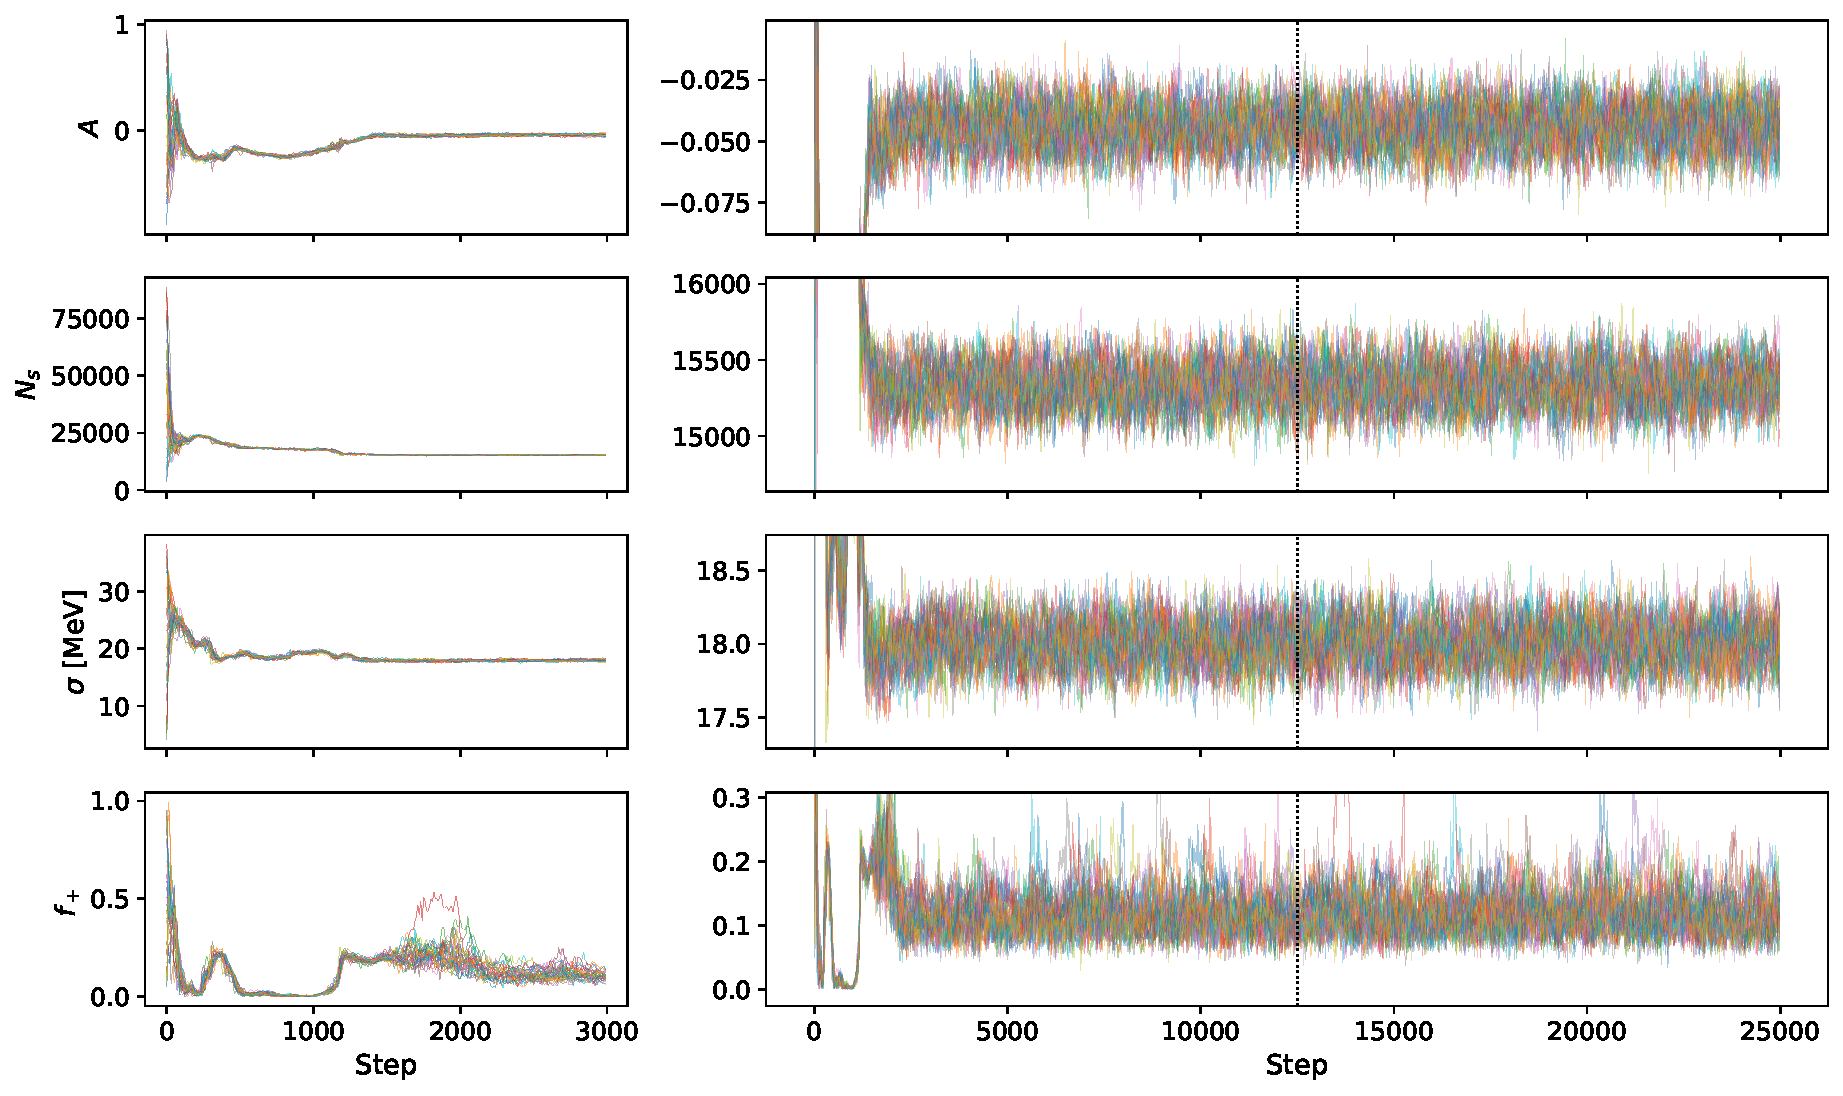
\includegraphics[width=0.95\textwidth]{figures/bayes_nominal_trace.pdf}
\caption{Trace plot of the nominal fit with the 32 walkers initialized uniformly over the prior box (one line per walker, every 10th step), for $A$, $N_s$, $\sigma$ and the steep-background fraction $f_+$. Left: first 3000 steps, full range; right: whole chain, zoomed on the posterior. The first half of the chain (dotted line) is discarded as burn-in.}
\label{fig:bayes_trace}
\end{figure*}

\begin{table*}[t]
\centering
\begin{tabular}{lp{7cm}lc}
\toprule
Model & Grid & Best configuration & CV AUC / Test AUC (default) \\
\midrule
Random Forest & \texttt{n\_estimators} $200$--$1200$, \texttt{max\_depth} $6$--$12$ or none, \texttt{min\_samples\_leaf} $5$--$40$ & $400$, $12$, $5$ & $0.8706$ / $0.8656$ ($0.8604$) \\
Gradient Boosting & \texttt{n\_estimators} $100$--$500$, \texttt{max\_depth} $1$--$5$, \texttt{learning\_rate} $0.01$--$0.1$ & $300$, $2$, $0.1$ & $0.8684$ / $0.8650$ ($0.8643$) \\
\bottomrule
\end{tabular}
\caption{Hyperparameter search for the tree ensembles ($120$ and $100$ configurations, 5-fold cross-validation repeated 10 times, balanced class weights). The test AUC of the best configuration is compared with that of the default of Table~\ref{tab:ml_models} (in parentheses); the bootstrap uncertainty of each test AUC is $0.012$.}
\label{tab:ml_hyperparams}
\end{table*}

\begin{table*}[t]
\centering
\begin{tabular}{llccc}
\toprule
Architecture & Layers & Dropout & Learning rate & CV AUC \\
\midrule
\texttt{deep\_3layer} (best) & $[64,32,16]$ & $0.2$ & $0.003$ & $0.8585\pm0.0174$ \\
\texttt{wide\_2layer}        & $[64,32]$    & $0.3$ & $0.003$ & $0.8582\pm0.0175$ \\
\texttt{deep\_3layer}        & $[64,32,16]$ & $0.3$ & $0.003$ & $0.8580\pm0.0187$ \\
\texttt{wide\_2layer}        & $[64,32]$    & $0.3$ & $0.005$ & $0.8579\pm0.0184$ \\
\texttt{wide\_2layer}        & $[64,32]$    & $0.4$ & $0.005$ & $0.8579\pm0.0187$ \\
\bottomrule
\end{tabular}
\caption{Top five of the $168$ FFNN configurations ($7$ architectures from one hidden layer of 8 units to five layers $[128,64,32,16,8]$, dropout $0.1$--$0.4$, learning rates $0.0002$--$0.005$; 5-fold cross-validation repeated twice). The five are within $0.0007$ of each other, far below the fold-to-fold spread: the optimum is a plateau. The best configuration has test AUC $0.8606$, against $0.8568$ for the default architecture ($\pm0.005$ over initializations).}
\label{tab:ml_ffnn_search}
\end{table*}

\section{Frequentist Quantities Used in the Text}
\label{sec:appendix_freq}
This appendix states in plain terms what the frequentist uncertainties and the test of $A=0$ are (Sec.~\ref{sec:frequentist}).

\paragraph{Hesse uncertainties.}
For $n$ independent candidates the likelihood contains the information on the parameters $\theta$ through the Fisher information matrix, $I_{ij}=-E\big[\partial^2\ln L/\partial\theta_i\partial\theta_j\big]$. The information inequality (minimum variance bound) states that the variance of an estimator cannot be smaller than the inverse of $I$ (for an unbiased one), and the maximum-likelihood estimate reaches the bound asymptotically, where it is also unbiased and Gaussian~\cite{cowan}. The covariance matrix of the fit is therefore $V\simeq I^{-1}$ evaluated at the best-fit point, with the second derivatives of $-\ln L$ computed numerically: this is the Hesse matrix of \texttt{iminuit}, and $\sigma(A)=0.0085$ is the square root of the diagonal element of $V$ for $A$, which includes the effect of the eleven nuisance parameters. It assumes that $-\ln L$ is parabolic around the minimum. The Minos intervals do not: they follow the profile likelihood on each side of the minimum, and their agreement with the Hesse error ($-0.0085$, $+0.0085$) shows that the parabola is a good description here.

\paragraph{Test of $A=0$.}
The null hypothesis $H_0$: $A=0$ is tested against the alternative $H_1$: $A$ free, the other parameters being free in both. The test statistic is the profile likelihood ratio,
$q(0)=-2\ln\big[L(0,\hat{\hat\theta})/L(\hat A,\hat\theta)\big]=2\Delta\mathrm{NLL}$, large when the data disfavor $H_0$. For two simple hypotheses the likelihood ratio is the most powerful test of a given size, i.e.\ the one with the highest probability of rejecting $H_0$ when $H_1$ is true (Neyman-Pearson lemma~\cite{neyman_pearson}); the profile likelihood ratio is its extension to hypotheses with unspecified parameters, with no optimality guarantee in general. By Wilks' theorem~\cite{wilks}, under $H_0$ the statistic follows a $\chi^2$ distribution with one degree of freedom, the number of parameters fixed by $H_0$, whatever the number of nuisance parameters, so the $p$-value is $P(\chi^2_1\geq q_{\mathrm{obs}})$; this is the probability, under $H_0$, of a result at least as discrepant as the data, not the probability of $H_0$.

\paragraph{Significance.}
A $\chi^2_1$ variable is the square of a standard normal one, so $p=P(|N|\geq\sqrt{q})$ and the significance quoted is $Z=\sqrt{q(0)}$ ($q\simeq27$, $p=2.05\times10^{-7}$, $Z=5.20$). This is a two-sided convention: the one-sided one, $Z=\Phi^{-1}(1-p)$, applied to the same $p$ would give $5.06$. For a parabolic likelihood $\sqrt{q}$ coincides with the Hesse significance $|\hat A|/\sigma(A)=5.19$.
